\section{半监督分类}
\label{sec:classification-semisupervised}

前面介绍的分类器依靠带标签的样本选择决策边界，但能够收集到的输入往往多于能够完成标注的样本。例如，积累一批待分类文档相对容易，逐篇判断主题却需要人工阅读。如果只使用已经标注的少量文档，其余文档所反映的词语共现和主题聚集结构就没有参与学习。\term{半监督分类}（semi-supervised classification）试图利用这部分信息：由真实标签确定类别含义，再借助未标注输入约束预测规则。

本节把全部$n$个样本的索引分成不相交的有标签集合$L$与无标签集合$U$，满足$L\cup U=\{1,\dots,n\}$。每个输入为$\bm{x}_i\in\mathbb{R}^{d}$，只有$i\in L$时可以在训练中使用真实标签$y_i$；除二分类的专门约定外，类别取值为$\{1,\dots,C\}$。这里的“无标签”描述算法可用的信息，不表示样本在真实任务中没有类别。标签稀缺是学习条件，树、概率模型和间隔模型则描述怎样表示或学习分类规则，因而半监督方法可以与前面几节的模型组合使用。

输入结构与类别之间的联系决定未标注数据能提供什么帮助。同样的两团文档，可能对应两个主题，也可能只因写作风格不同而聚集。分布不匹配、标签采样偏差或未知类别混入，都可能使采用的结构假设失效。Cozman与Cohen对生成式分类器的分析表明，生成模型失配时，加入未标注数据可能增大渐近偏差和分类错误\scite{cozman2002unlabeled}。其结论限定于所分析的生成式模型，指出了核对结构假设的必要性。

Self-Training将筛选后的模型预测作为补充监督，Label Propagation沿相似关系平滑标签得分，TSVM利用输入密度选择间隔边界。三种机制可以共享条件，也可以组合。下面分别说明未标注输入怎样进入训练、目标怎样求解，以及哪些分布联系支撑样本外收益。

\subsection{Self-Training}
\label{sec:classification-self-training}

已经用少量标注文档训练出一个分类器以后，可以先让它预测其余文档。例如，模型对某些包含已知主题词的文档有较高置信度，而这些文档还包含原标注集中少见的其他词。若采纳的类别判断可靠，重新训练就能把这些新词与已有类别联系起来，扩展原来的标签覆盖。

\term{自训练}（self-training）将这个思路组织成外层循环：基分类器产生预测，外层策略筛选部分预测作为补充标签，再扩充训练集并重新拟合。它复用已有分类器，新增的是筛选与重训机制。高置信度也可能来自模型的错误偏好，后面需要检查采纳规则及错误反馈。用机器自身的输出代替部分教师信号的思想，在Scudder于1965年研究的自适应模式识别方法中已经出现；现代筛选、加权和重训方式则可以有许多实现\scite{scudder1965selftraining}。

\subsubsection{模型结构}
\label{sec:classification-self-training-structure}

自训练不要求一种新的决策边界形式。基分类器仍可采用Logistic回归、SVM、决策树或随机森林；新增的部分是怎样管理暂时没有真实标签的样本。为了不混淆真实监督与模型生成的监督，保持原始$L$和$U$不变，用$A^{(t)}\subseteq U$记录第$t$轮已经采纳伪标签的样本索引，用$R^{(t)}=U\setminus A^{(t)}$记录剩余候选池。初始时$A^{(0)}=\varnothing$，模型只在$L$上训练。

假设基分类器以参数$\bm{\theta}$给出类别概率估计$p_{\bm{\theta}}(c\mid\bm{x})$。本节讨论一种阈值筛选方式，把最大类别概率作为\term{置信度}（confidence），即模型对自己当前分类结果的确定程度。对$j\in R^{(t)}$，计算
\begin{equation}
  \label{eq:classification-self-training-selection}
  \begin{aligned}
    \widehat y_j^{(t)}
      &=\argmax_{1\leq c\leq C}
        p_{\bm{\theta}^{(t)}}(c\mid\bm{x}_j),\\
    q_j^{(t)}
      &=\max_{1\leq c\leq C}
        p_{\bm{\theta}^{(t)}}(c\mid\bm{x}_j),\\
    B^{(t)}
      &=\{j\in R^{(t)}:q_j^{(t)}\geq\tau\}.
  \end{aligned}
\end{equation}
其中$\tau$是预先选择的阈值，通常取$1/C<\tau<1$；遇到并列最大值时，本节统一取编号最小的类别。被采纳的预测$\widetilde y_j=\widehat y_j^{(t)}$称为\term{伪标签}（pseudo-label）：它是模型提出的临时训练目标，并没有经过真实标注确认。本节的基本版本在采纳后固定该标签；允许重估或撤销伪标签的版本需要另外规定更新规则。

概率阈值要求筛选分数具有概率含义。SVM得分需先用独立标注数据建立并检验概率映射；直接输出概率的模型也需检查高置信度样本的实际错误率。例如二分类预测$(0.96,0.04)$满足$\tau=0.9$，$(0.55,0.45)$则被保留在候选池。采纳的是模型判为可靠的预测，真实标签仍待另行确认。

\subsubsection{参数学习}
\label{sec:classification-self-training-learning}

每轮采纳伪标签后，基分类器需要重新拟合。以可加权的损失$\ell$为例，当前训练目标可以写成
\begin{equation}
  \label{eq:classification-self-training-objective}
  \begin{aligned}
    \mathcal{J}_t(\bm{\theta})
      ={}&\frac{1}{|L|}\sum_{i\in L}
        \ell\bigl(f_{\bm{\theta}}(\bm{x}_i),y_i\bigr)\\
      &+\frac{\eta}{\max\{1,|A^{(t)}|\}}
        \sum_{j\in A^{(t)}}
        \ell\bigl(f_{\bm{\theta}}(\bm{x}_j),\widetilde y_j\bigr)\\
      &+\beta\Omega(\bm{\theta}).
  \end{aligned}
\end{equation}
这里$L$非空，$\eta\geq0$控制伪标签项的相对权重，$\beta\Omega$沿用基分类器的正则化方式。空伪标签集的求和取零。分别归一化两类样本，是为了避免仅因伪标签数量增加就让它们压过真实标签；若采用统一样本权重，其相对影响会随集合大小改变。对于树等不直接求解这个目标的分类器，可以使用对应的带权拟合接口，自训练的集合更新逻辑不变。

算法\ref{alg:classification-self-training}给出固定阈值、固定已采纳伪标签的版本。$\operatorname{Fit}(A)$表示用真实标签集与索引为$A$的伪标签集完成一次基分类器训练，并返回参数；式~\eqref{eq:classification-self-training-objective}~是这种训练的一种具体实现。算法中省略集合的迭代上标，始终让当前参数对应当前已采纳的训练集。

\begin{algorithm}[带最终重训的自训练]
  \label{alg:classification-self-training}
  \begin{algorithmic}[1]
    \Require 有标签索引$L$、无标签索引$U$及其输入
    \Require 阈值$\tau$、最大扩充轮数$T\geq0$
    \Ensure 分类器$f_{\bm{\theta}}$、已采纳索引$A$和剩余索引$R$
    \State $A\gets\varnothing$，$R\gets U$
    \State $\bm{\theta}\gets\operatorname{Fit}(A)$
    \For{$t=1,\dots,T$}
      \If{$R=\varnothing$}
        \State \textbf{break}
      \EndIf
      \State 用当前模型计算$R$中的$\widehat y_j$与$q_j$
      \State $B\gets\{j\in R:q_j\geq\tau\}$
      \If{$B=\varnothing$}
        \State \textbf{break}
      \EndIf
      \State 保存$\widetilde y_j\gets\widehat y_j$，$j\in B$
      \State $A\gets A\cup B$，$R\gets R\setminus B$
      \State $\bm{\theta}\gets\operatorname{Fit}(A)$
    \EndFor
    \State \Return $f_{\bm{\theta}},A,R$
  \end{algorithmic}
\end{algorithm}

把重训放在集合扩充之后有一个直接作用：无论这一轮恰好用完最大轮数，还是把剩余池清空，返回的模型都已经使用了本轮加入的伪标签。若把训练放在循环开头、随后只添加样本就退出，最后一批伪标签实际上不会影响返回模型。预测前检查空池也很必要，空输入未必被基分类器的批量预测接口接受。当$U$为空或$T=0$时，算法自然返回纯监督模型。

图\ref{fig:classification-self-training}中的反馈箭头将重训后的模型送回预测步骤。真实标签固定在$L$中，未采纳的样本保留在$R$，已采纳的预测保存在$A$；这些集合变化记录监督的来源，使每轮能够区分真实标签与模型生成的伪标签。

\begin{figure*}[htbp]
  \centering
  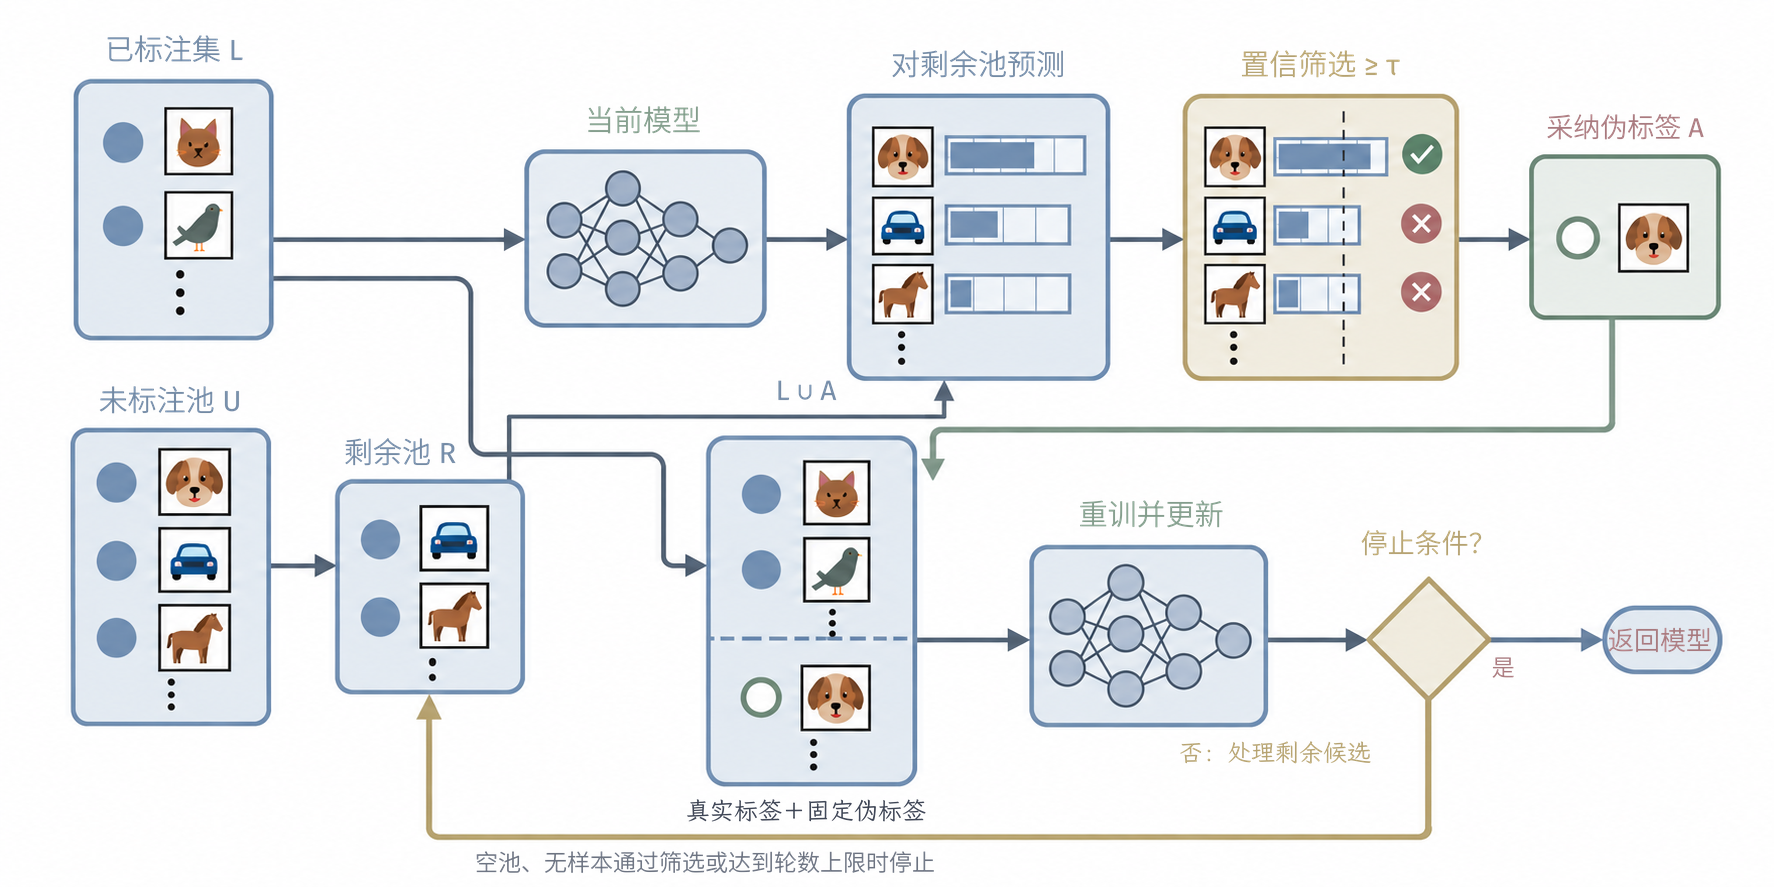
\includegraphics[width=150.199mm]{figures/04-classic-models/00-shared/generated/classification-self-training/figure.png}
  \caption{固定阈值、固定已采纳伪标签的自训练流程，对应算法~\ref{alg:classification-self-training}。真实标签保持不变，已采纳的伪标签始终是模型预测。每次采纳后先重训，再用更新后的模型处理剩余候选；空池、无样本通过筛选或达到轮数上限时停止。这个模型反馈回路也可能产生确认偏差：错误预测被当作后续监督，使模型进一步强化原有误判。}
  \label{fig:classification-self-training}
\end{figure*}

每轮也可以在通过阈值的样本中只取前若干项，限制一次扩充的影响；按类别限制数量则可避免易预测类别占据全部新增监督。这些策略改变$B^{(t)}$的构造，集合更新仍按保存标签、扩充集合、重训的顺序执行。类别配额依据任务中的类别比例设置。

\subsubsection{理论分析}
\label{sec:classification-self-training-analysis}

\paragraph{表达能力}
自训练沿用基分类器的特征与函数形式，候选类不会因增加伪标签而扩大。若基分类器只使用原坐标的仿射得分，前面的四点异或仍不能精确表示，等概率四点上的标签不一致比例至少为$1/4$。加入$x_1x_2$后，得分$-x_1x_2$才使这项目标进入候选类。

\paragraph{收敛性}
这个基本版本何时停止，可以直接从集合变化判断。每次成功扩充至少从$R$移走一个样本，且样本不会移回，因此成功扩充最多发生$\min\{T,|U|\}$次；若没有样本通过筛选，循环会更早结束。只要每次基分类器训练能够返回，外层循环就会有限终止。这一保证针对集合扩充过程的有限终止；各轮训练集和监督信号发生变化，参数优化与统计风险需针对相应模型另行分析。

自训练与\term{熵最小化}（entropy minimization）有共同的倾向：都可能让未标注样本上的预测变得更确定。熵最小化直接惩罚模型预测分布的条件熵，推动概率集中到少数类别。Grandvalet与Bengio讨论了这一准则及其与自训练的联系，这种联系依赖具体的概率模型、筛选和优化设置\scite{grandvalet2004entropy}。

对一个未标注输入$\bm{x}$，Shannon熵与硬伪标签交叉熵分别涉及
\begin{equation}
  \label{eq:classification-pseudolabel-entropy}
  \begin{aligned}
    H_{\bm{\theta}}(\bm{x})
      &=-\sum_{c=1}^{C}p_{\bm{\theta}}(c\mid\bm{x})
        \log p_{\bm{\theta}}(c\mid\bm{x}),\\
    \min_{\widetilde y\in\{1,\dots,C\}}
      \{-\log p_{\bm{\theta}}(\widetilde y\mid\bm{x})\}
      &=-\log\max_c p_{\bm{\theta}}(c\mid\bm{x}).
  \end{aligned}
\end{equation}
前者对所有类别求加权和，后者只取概率最大的一个类别，两者数值和梯度一般不同。例如，预测为$(0.8,0.2)$时，以自然对数计算的熵约为$0.500$，最小硬标签交叉熵约为$0.223$。实际自训练还会筛选样本并冻结历史伪标签，因此下一轮甚至不一定仍以当前最大概率类别为目标。

\paragraph{泛化性}
在同一聚集区域内限制预测差异时，熵最小化倾向于同时提高这些输入的确定性，使边界远离该区域；具体效果依赖基分类器的容量与约束方式。确定性本身仍只描述概率集中程度：若初始模型把同主题文档误判为另一类，采纳后重训可能加强原误判。这种自身错误被重复用作监督的现象称为\term{确认偏差}（confirmation bias）。Arazo等在深度图像分类实验中观察到错误伪标签被拟合，并比较了缓解这一反馈的正则化方法\scite{arazo2020confirmation}。

伪标签错误怎样影响真实风险，可以在固定一轮模型后直接推导。令$h$为这一轮产生伪标签的分类器，$\bm{X}_\tau\subseteq\mathbb{R}^{d}$为通过其置信度阈值的输入区域；$R_{\mathcal P}$沿用目标分布上的零一风险记号。设$\pi=\mathbb{P}_{\mathcal{P}}(\bm{x}\in\bm{X}_\tau)>0$，在筛选区域内分别考察伪标签自身的错误率，以及$f$与伪标签不一致的概率：
\begin{equation}
  \label{eq:classification-self-training-conditional-risks}
  \begin{aligned}
    e_\tau
      &=\mathbb{P}_{\mathcal{P}}
        \bigl(h(\bm{x})\ne y\mid\bm{x}\in\bm{X}_\tau\bigr),\\
    \widetilde R_\tau(f)
      &=\mathbb{P}_{\mathcal{P}}
        \bigl(f(\bm{x})\ne h(\bm{x})\mid\bm{x}\in\bm{X}_\tau\bigr).
  \end{aligned}
\end{equation}
若$f$预测错误，它要么与$h$不一致，要么沿用了$h$的错误，因此
\begin{equation}
  \label{eq:classification-self-training-error-events}
  \{f(\bm{x})\ne y\}
    \subseteq
    \{f(\bm{x})\ne h(\bm{x})\}
    \cup\{h(\bm{x})\ne y\},
\end{equation}
在$\bm{X}_\tau$内应用并集界，再把区域内外的风险相加，得到
\begin{equation}
  \label{eq:classification-self-training-risk}
  \begin{aligned}
    R_{\mathcal{P}}(f)
      \leq{}&\pi\bigl(\widetilde R_\tau(f)+e_\tau\bigr)\\
      &+\mathbb{P}_{\mathcal{P}}
        \bigl(f(\bm{x})\ne y,\ \bm{x}\notin\bm{X}_\tau\bigr).
  \end{aligned}
\end{equation}
式~\eqref{eq:classification-self-training-risk}中的$\widetilde R_\tau(f)$仍是期望不一致损失，不能用训练伪标签上的错误直接替换。若产生标签的模型与新输入池独立，可以把这一步也写成风险界。
\begin{theorem}[自训练在独立输入池与固定候选类下的期望风险界]
  \label{thm:classification-self-training-risk}
  条件于已经训练好的$h$，固定筛选区域$\bm X_\tau$，并在采集本轮伪标签输入前固定含$N\geq1$个分类器的候选类$\mathcal F$。独立抽取$m\geq1$个来自$P_X(\cdot\mid\bm X_\tau)$的输入，以$h$的预测为标签。学习器用这些样本和已有监督返回$\hat f\in\mathcal F$，记其本轮伪标签训练错误为
  \[
    \widehat R_{\mathrm{pseudo}}(\hat f)
      =\frac1m\sum_{j=1}^m
        \mathbb1\{\hat f(\bm x_j)\ne h(\bm x_j)\}.
  \]
  对$0<\delta<1$，关于本轮输入抽样，至少以$1-\delta$的概率，
  \[
    R_{\mathcal P}(\hat f)
      \leq\pi\left[
        \widehat R_{\mathrm{pseudo}}(\hat f)+e_\tau
        +\sqrt{\frac{\log(2N/\delta)}{2m}}\right]
       +(1-\pi).
  \]
\end{theorem}
\begin{proof}
  固定$h$以后，与其伪标签不一致的损失取值于$[0,1]$，其期望是$\widetilde R_\tau(f)$。对本轮独立样本和预定候选类使用有限类的一致偏差界，得到
  $\widetilde R_\tau(\hat f)\leq\widehat R_{\mathrm{pseudo}}(\hat f)
       +\sqrt{\log(2N/\delta)/(2m)}$。
  代入式\eqref{eq:classification-self-training-risk}，再用$1-\pi$上界区域外错误，即得结论。
\end{proof}

这说明即使重训模型完全拟合伪标签，仍要保留采纳区域中的真实错误$e_\tau$和区域外风险。较高的概率阈值本身不提供$e_\tau$的上界；它需要可靠的概率条件或独立真实标签来支持。定理分析的是一轮固定教师、独立输入池和有限候选类；连续参数基模型需要相应容量界。多轮使用同一输入池时，历史伪标签来自不同模型与采纳事件，不能把累积伪标签数直接当作这里的独立样本数$m$。

提高阈值减少采纳量，系统性的高置信度错误仍可能被保留。伪标签权重与单轮规模控制其训练影响，逐类接受率揭示扩充偏向，保留的真实标签验证集则比较扩充前后的效果。验证样本应独立于反复采纳的训练池。未知类别或监督样本覆盖不足时，还需检查数据组成与筛选区域是否符合任务。

\subsubsection{优化泛化能力}

\paragraph{保留未标注类别的不确定性}
\label{sec:classification-self-training-soft-em}

自训练将筛选后的类别作为确定标签；若基分类器已经建立NB或高斯类条件分布，还可以保留类别的不确定性，改用联合似然组织训练。例如，一篇文档当前可能有较高概率属于科技，也有一定概率属于文化，与其立即固定成科技类，不如按两类的后验权重分配它的词频贡献，并在参数更新后重新计算归属。这是生成式半监督方法用潜类别与EM利用未标注输入的路线。它与筛选硬伪标签的自训练使用不同训练目标，不是简单地把筛选阈值调低。

设联合模型为$p_{\bm{\theta}}(\bm{x},y)$，有标签样本直接贡献输入与类别的联合对数似然，未标注样本则只贡献输入的边缘对数似然：
\[
  \ell(\bm{\theta})
  =\sum_{i\in L}\log p_{\bm{\theta}}(\bm{x}_i,y_i)
   +\sum_{j\in U}\log\sum_{c=1}^{C}
      p_{\bm{\theta}}(\bm{x}_j,c).
\]
在这个模型中，全部输入与全部类别合称\term{完全数据}（complete data），其中包括实际未观测的类别；这里的“完全”指连同潜类别一并规定的随机变量。EM在训练时把$U$中的未知类别作为潜变量处理。E步用当前参数计算软后验$q_j(c)=p_{\bm{\theta}^{(t)}}(y=c\mid\bm{x}_j)$；M步最大化当前软后验下的期望完全数据对数似然。记
\[
  \begin{aligned}
    Q(\bm{\theta}\mid\bm{\theta}^{(t)})
    &=
    \sum_{i\in L}\log p_{\bm{\theta}}(\bm{x}_i,y_i) \\
    &\quad+
    \sum_{j\in U}\sum_{c=1}^{C}
      q_j(c)\log p_{\bm{\theta}}(\bm{x}_j,c), \\
    \bm{\theta}^{(t+1)}
    &\in\argmax_{\bm{\theta}}
      Q(\bm{\theta}\mid\bm{\theta}^{(t)}).
  \end{aligned}
\]
只有对多项式NB这类以类别与类别词频为充分统计量的模型，M步才可以解释为把$q_j(c)$作为分数类别计数，与真实标签统计量一起更新先验和类条件参数。此时，未标注文档的词频按$q_j(c)$分配给各类别，而不是先固定成一个不可更改的硬伪标签。Nigam等在文本分类中给出了这一路线的代表性实现\scite{nigam2000text}。

EM改变估计过程，联合分布仍限于预定的$p_{\bm\theta}(\bm x,y)$。选多项式NB就仍使用加性的词频证据，选每类单个高斯就仍不能表达任意多峰类内分布；未标注数据不会替模型补上缺少的依赖项。分布族能够表达真实联合分布时，软类别统计量才有对应的目标参数；这与EM是否找到全局似然最大点仍是两个问题。

模型失配时，大量未标注输入可能加强对错误边缘结构的拟合；Cozman与Cohen对分类性能劣于监督基线的现象给出了分析与实验\scite{cozman2002unlabeled}。后验不能闭式计算时，近似推断又增加了一层误差与计算选择；相应图模型入口见\BookVolumeRef{vol:probabilistic-graphical-models}{卷六“模型：概率图模型”}。

\paragraph{降低伪标签对单个教师的依赖}
同一个模型提出并采纳标签时，系统性偏差可能被重复使用。若输入具有两种各自足以分类的描述，Blum与Mitchell在1998年提出的\term{协同训练}（co-training）可以让两个视图的分类器互供候选标签；其理论设定还要求给定类别后的视图条件独立。没有这种视图关系时，互供标签也可能传播共同错误，且需要训练和评价两个模型\scite{blum1998cotraining}。

没有两种天然视图时，Zhou与Li在2005年提出的\term{三训练}（tri-training）用重采样初始化三个模型，让两个模型的一致预测为第三个提供候选标签，并控制新增标签的错误负担。这增加了模型训练和预测成本，一致意见是否有用仍取决于错误相关性；它改变了监督来源，不是单模型自训练的一项默认设置\scite{zhou2005tritraining}。

\subsubsection{小结}
\label{sec:classification-self-training-summary}

自训练把已有分类器的部分预测转化为新增监督，适合在保留原有训练和预测接口的情况下探索无标签数据的价值。它的额外成本包括对剩余池反复预测，以及在不断扩大的训练集上重新拟合；基分类器训练昂贵时，这些成本并不小。最终模型仍按原分类器的方式预测新样本，无须保留一个独立的传播图。

硬伪标签把当前判断作为后续监督，生成式EM则按当前软类别归属分配统计量，并反复更新联合模型。前者依赖筛选是否可靠，后者还依赖输入分布是否被模型正确描述；两者都可能把错误结构反复写入训练。保留真实标签验证集和针对高代价样本的人工复核，有助于判断新增监督是否值得采纳。

互供标签改变的是新增监督从哪里来。协同训练依靠不同视图，三训练依靠多个模型的一致判断；它们需要更多模型的训练和预测，也要检查共同错误是否被反复采纳。软类别归属与多模型监督来源因此是两个可以分别考虑的方向，不构成由简单到复杂的性能排序。

\subsection{Label Propagation}
\label{sec:classification-label-propagation}

自训练通过基分类器决定哪些预测值得采纳；如果可信的信息主要来自样本之间的邻近关系，也可以直接在这些关系上传递标签。\term{标签传播}（label propagation）把样本表示为图的节点，让已有标签沿相似边影响尚无标签的节点。Zhu与Ghahramani在2002年的技术报告中给出了保持已知标签不变的传播方法\scite{zhu2002labelpropagation}。与只在已标注样本中寻找近邻相比，未标注点也参与形成传播路径，使标签能够沿弯曲的高密度区域传递；每轮恢复已知标签，则让它们持续提供监督，不会因反复平均而失去原有的类别信息。

下面用随机游走解释固定标签边界下的传播，软约束版本随后通过另一目标引入。

\subsubsection{模型结构}
\label{sec:classification-label-propagation-structure}

图模型把“哪些输入相似”转化成可计算的边权。令$\mathcal{G}=(V,E,\bm{W})$，其中$V=L\cup U$，$\bm{W}\in\mathbb{R}^{n\times n}$为非负对称权重矩阵，$\bm{W}_{i,j}=\bm{W}_{j,i}\geq0$，且取$\bm{W}_{i,i}=0$。例如，可以先选出近邻边，再在相连节点上使用RBF相似度
\begin{equation}
  \label{eq:classification-label-propagation-weights}
  \bm{W}_{i,j}=
  \begin{cases}
    \exp\bigl(-\gamma\lVert\bm{x}_i-\bm{x}_j\rVert_2^2\bigr),
      & \{i,j\}\in E,\\
    0, & \text{其他情形},
  \end{cases}
\end{equation}
其中$\gamma>0$控制相似度衰减。用$k$近邻关系构图时，单向近邻关系需要经过并集或互近邻等明确规则转成无向边，才能满足对称性。完全图保留所有样本对，稀疏图只保留选中的关系；两者不仅存储成本不同，也可能给出不同的分类结果。

每个节点的加权度记为$\delta_i=\sum_j\bm{W}_{i,j}$，度矩阵满足$\bm{D}_{i,i}=\delta_i$。在所有参与传播的节点度数为正时，定义
\begin{equation}
  \label{eq:classification-label-propagation-transition}
  \bm{P}=\bm{D}^{-1}\bm{W},
  \qquad
  \bm{P}_{i,j}=\frac{\bm{W}_{i,j}}{\delta_i}.
\end{equation}
矩阵$\bm{P}$每行的和为1，表示从一个节点沿边随机走向邻居的转移概率。传播时用这一行权重对邻居的标签信息求平均；权重大，邻居的影响也大。

为了同时处理$C$个类别，令$\bm{F}\in\mathbb{R}^{n\times C}$保存节点得分，$\bm{f}_i=(\bm{F}_{i,1},\dots,\bm{F}_{i,C})^\top$为节点$i$的得分向量。构造同形状的$\bm{Y}$：若$i\in L$，则$\bm{Y}_{i,c}=\mathbb{1}\{y_i=c\}$；若$i\in U$，则整行置零。有标签节点在每轮更新后都恢复到这份独热编码，这种固定边界的操作称为\term{硬钳制}（hard clamping），也就是不允许传播改变已经给定的标签。

标签边界应能沿图到达每个待预测节点。零度无标签节点没有转移概率，完全无标签的连通分量则缺少类别语义；可补充真实标签、按可靠关系重新构图，或对相应节点拒绝预测。孤立的有标签节点保留原标签。自环或微小度数只能调整数值形式，类别信息仍需要标签边界提供。

\subsubsection{参数学习}
\label{sec:classification-label-propagation-learning}

标签传播没有固定维数的分类器参数要拟合，但需要求出全部无标签节点的得分。下面假设零度节点已经处理，每个含无标签节点的连通分量至少含一个有标签节点。把$\bm{F}$按$L$与$U$分成行块$\bm{F}_L=\bm{F}_{L,:}$、$\bm{F}_U=\bm{F}_{U,:}$，并对$\bm{P}$作对应分块。硬钳制意味着$\bm{F}_L^{(t)}=\bm{Y}_L$始终不变，因而只需迭代
\begin{equation}
  \label{eq:classification-label-propagation-iteration}
  \bm{F}_U^{(t+1)}
    =\bm{P}_{U,U}\bm{F}_U^{(t)}
     +\bm{P}_{U,L}\bm{Y}_L.
\end{equation}
右侧第一项传递尚无标签节点之间的当前信息，第二项持续注入真实标签。通常取$\bm{F}_U^{(0)}=\bm{0}$。真实标签在每轮固定为边界，无标签行按该转移式更新。

若迭代达到固定点，移项便得到线性系统与形式上的闭式解
\begin{equation}
  \label{eq:classification-label-propagation-solution}
  \begin{aligned}
    (\bm{I}-\bm{P}_{U,U})\bm{F}_U^\ast
      &=\bm{P}_{U,L}\bm{Y}_L,\\
    \bm{F}_U^\ast
      &=(\bm{I}-\bm{P}_{U,U})^{-1}
        \bm{P}_{U,L}\bm{Y}_L.
  \end{aligned}
\end{equation}
这里$\bm{I}$为$|U|\times|U|$单位矩阵。本节理论分析将证明，在上述图条件下逆矩阵存在，且任意初始化的迭代都收敛到同一个解。计算时通常直接求解线性系统，避免显式构造逆矩阵。Zhu、Ghahramani与Lafferty给出了这一解的调和函数、图能量和随机游走解释\scite{zhu2003}。

图\ref{fig:classification-label-propagation}给出一个可逐项核算的教学构造，并非实测数据。五个节点依次相连，每条无向边的权重为1；端点1固定属于类1，端点5固定属于类2，节点2、3、4没有标签。令$p_i=\bm{F}_{i,1}^\ast$，由于每个内点恰有两个等权邻居，式~\eqref{eq:classification-label-propagation-iteration}~在固定点处变为
\begin{equation}
  \label{eq:classification-label-propagation-path}
  \begin{aligned}
    p_i&=\frac{p_{i-1}+p_{i+1}}{2},
      &&i=2,3,4,\\
    p_1&=1,\qquad p_5=0.
  \end{aligned}
\end{equation}
内点方程等价于$p_{i+1}-p_i=p_i-p_{i-1}$，所以相邻节点的得分差必须相等。两端总共下降1，分到四条边上，每步下降$1/4$，得到
\[
  (p_1,p_2,p_3,p_4,p_5)
    =(1,0.75,0.5,0.25,0).
\]
类2的得分满足相反的端点条件，故$\bm{f}_i^\ast=(p_i,1-p_i)^\top$。节点2偏向类1，节点4偏向类2；节点3的两类得分相同，按本节“并列时取最小类别编号”的约定判为类1。节点3的类别由并列规则确定，其两类得分所包含的证据仍相同。

\begin{figure}[htbp]
  \centering
  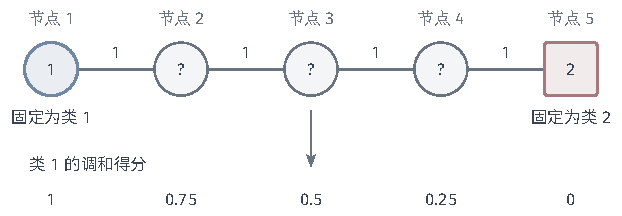
\includegraphics[width=105.315mm]{figures/04-classic-models/00-shared/tikz/classification-label-propagation/figure.pdf}
  \caption{五节点等权无向路径上的硬钳制标签传播。每条边权为1，左端圆形节点固定为类1，右端方形节点固定为类2，问号表示未知标签。下方列出精确调和解的类1得分，类2得分为其补数；内点得分等于两侧邻居的平均。中间节点两类并列，按最小类别编号规则判为类1。这是教学构造，不是实测结果。}
  \label{fig:classification-label-propagation}
\end{figure}

迭代实现还需要把停止条件与返回值对应起来。算法\ref{alg:classification-label-propagation}使用相邻两轮之差作为数值停止判据，其中$\lVert\cdot\rVert_{\mathrm{F}}$为Frobenius范数，$\varepsilon>0$为容限，$T\geq1$为最大迭代次数。达到上限时若尚未满足容限，返回状态记录为未收敛，以便解释当前得分的数值精度。

\begin{algorithm}[硬钳制标签传播]
  \label{alg:classification-label-propagation}
  \begin{algorithmic}[1]
    \Require 权重$\bm{W}$、索引$L,U$、标签矩阵$\bm{Y}$
    \Require 容限$\varepsilon>0$、最大迭代次数$T\geq1$
    \Ensure 得分$\bm{F}$、预测$\widehat{\bm{y}}_U$及停止状态
    \If{$U=\varnothing$}
      \State \Return $\bm{Y}$、空预测、已完成
    \EndIf
    \State 检查$\bm{W}$非负、对称，参与传播的节点度数为正
    \State 检查每个含$U$节点的连通分量至少有一个$L$节点
    \If{任何检查失败}
      \State \Return 拒绝结果，要求补标签或修正传播图
    \EndIf
    \State 构造$\bm{P}=\bm{D}^{-1}\bm{W}$
    \State $\bm{F}_L\gets\bm{Y}_L$，$\bm{F}_U\gets\bm{0}$
    \State $\mathrm{converged}\gets\mathrm{false}$
    \For{$t=1,\dots,T$}
      \State $\bm{G}\gets\bm{P}_{U,U}\bm{F}_U+\bm{P}_{U,L}\bm{Y}_L$
      \State $\Delta\gets\lVert\bm{G}-\bm{F}_U\rVert_{\mathrm{F}}$
      \State $\bm{F}_U\gets\bm{G}$
      \If{$\Delta\leq\varepsilon(1+\lVert\bm{F}_U\rVert_{\mathrm{F}})$}
        \State $\mathrm{converged}\gets\mathrm{true}$
        \State \textbf{break}
      \EndIf
    \EndFor
    \State $\widehat y_j\gets\argmax_c\bm{F}_{j,c}$，$j\in U$；并列取最小$c$
    \State \Return $\bm{F},\widehat{\bm{y}}_U,\mathrm{converged}$
  \end{algorithmic}
\end{algorithm}

算法先把$\bm{G}$保存成最新的$\bm{F}_U$，再判断是否退出，因此即使本轮达到容限，也会返回新得分而不是上一轮的值。相邻迭代差小是一种可操作的停止指标，不直接给出距离精确解的统一误差界；当传播很慢时，还需结合线性系统残差与条件数判断数值精度。最终类别由得分比较决定，接近平局的节点尤其需要保留得分与未收敛状态。

\subsubsection{理论分析}
\label{sec:classification-label-propagation-analysis}

\paragraph{表达能力}
固定图与标签边界时，硬钳制传播的候选得分须满足离散调和条件：标签节点保留给定得分，每个无标签节点的得分等于邻居得分的加权平均。若每个连通分量的真实类别都相同，且给定标签均正确，相应的常值独热得分就满足全部条件，目标因此在这个候选集合中，即使这些分量在原坐标中弯曲。

强连接中的交替标签则可能无法表达。例如，四个节点按$0,1,2,3$组成单位边权路径，节点0的标签为类1、节点3为类2。调和条件迫使两个内部节点的类2得分分别为$1/3$与$2/3$。按最大得分取类，它们只能分别归为类1和类2；若目标类别沿路径依次为1、2、1、2，两个内部节点便都与目标不一致。这一差距来自调和约束，目标所需的交替变化不在候选得分中。

\paragraph{收敛性}
硬钳制传播的收敛来自无标签节点能够沿正权路径到达标签边界。$\bm{P}_{U,U}$的行和至多为1，只有无标签邻居的节点其行和恰为1。因此考察多步后仍留在$U$中的总权重，可以同时处理直接与间接相连的节点。

\begin{theorem}[标签传播在各连通分量有标签条件下解的唯一性]
  \label{thm:classification-label-propagation-convergence}
  设图有限、边权非负且对称，所有参与传播的节点度数为正，$U$非空，且每个含无标签节点的连通分量至少含一个有标签节点。则$\rho(\bm{P}_{U,U})<1$，其中$\rho$表示谱半径。式~\eqref{eq:classification-label-propagation-iteration}~从任意初始得分出发，都收敛到式~\eqref{eq:classification-label-propagation-solution}~中的唯一固定点。
\end{theorem}

\begin{proof}
  从每个$j\in U$出发，选择一条到达$L$的正权路径，并在首次到达$L$时停止。有限图中这些路径长度有一个共同上界$m$，沿各路径行走的概率均为正，其最小值记为$\epsilon>0$。于是，无论从哪个无标签节点出发，在$m$步以内命中$L$的概率都至少为$\epsilon$。这说明
  \[
    \lVert\bm{P}_{U,U}^{m}\rVert_\infty\leq1-\epsilon,
    \qquad
    \rho(\bm{P}_{U,U})^m\leq1-\epsilon<1.
  \]
  因而$\bm{P}_{U,U}^t$趋于零，Neumann级数收敛，且
  \[
    (\bm{I}-\bm{P}_{U,U})^{-1}
      =\sum_{t=0}^{\infty}\bm{P}_{U,U}^{t}.
  \]
  迭代展开为
  \[
    \bm{F}_U^{(t)}
      =\bm{P}_{U,U}^{t}\bm{F}_U^{(0)}
       +\sum_{s=0}^{t-1}
         \bm{P}_{U,U}^{s}\bm{P}_{U,L}\bm{Y}_L.
  \]
  第一项消失，第二项趋于所述固定点。逆矩阵存在，也排除了其他固定点。
\end{proof}

还可以从最优化的角度解释同一个解。相邻节点的得分差越大，图上的不平滑程度越高。令$\bm{L}_{\mathrm{g}}=\bm{D}-\bm{W}$为\term{图拉普拉斯矩阵}（graph Laplacian），它把这种局部差异汇总成二次型。固定真实标签边界后，求解的\term{Dirichlet能量}（Dirichlet energy）最小化问题为
\begin{equation}
  \label{eq:classification-label-propagation-energy}
  \begin{aligned}
    \min_{\bm{F}:\,\bm{F}_L=\bm{Y}_L}\quad
    \mathcal{E}(\bm{F})
      &=\frac12\sum_{i,j=1}^{n}
        \bm{W}_{i,j}\lVert\bm{f}_i-\bm{f}_j\rVert_2^2\\
      &=\operatorname{tr}
        (\bm{F}^{\top}\bm{L}_{\mathrm{g}}\bm{F}).
  \end{aligned}
\end{equation}
第\ref{sec:clustering-spectral}节的谱聚类与第\ref{sec:dim-le}节的拉普拉斯特征映射复用图拉普拉斯和谱工具，但输出分别是离散簇分配与连续低维坐标；这里的标签传播则在已知类别语义下求类别得分。三种任务分别对类别得分、簇分配和坐标施加输出约束。

有标签节点固定为边界，优化变量只包含无标签行。对未知行块求导并令其为零，得到
\begin{equation}
  \label{eq:classification-label-propagation-dirichlet}
  \begin{aligned}
    (\bm{L}_{\mathrm{g}})_{U,U}\bm{F}_U
      &=-(\bm{L}_{\mathrm{g}})_{U,L}\bm{Y}_L\\
      &=\bm{W}_{U,L}\bm{Y}_L.
  \end{aligned}
\end{equation}
因为$(\bm{L}_{\mathrm{g}})_{U,U}=\bm{D}_{U,U}-\bm{W}_{U,U}$，左乘$\bm{D}_{U,U}^{-1}$就回到式~\eqref{eq:classification-label-propagation-solution}~的线性系统。

这个驻点也是唯一最小值，而不只是一个形式上的导数解。取任意无标签节点上的非零向量$\bm{z}$，把它扩展成在$L$上为零的全图向量$\widetilde{\bm{z}}$，则
\[
  \bm{z}^{\top}(\bm{L}_{\mathrm{g}})_{U,U}\bm{z}
    =\frac12\sum_{i,j}\bm{W}_{i,j}
      (\widetilde z_i-\widetilde z_j)^2.
\]
右侧若为零，向量在每个正权连通分量上就必须为常数。每个涉及$U$的分量又含一个值为零的标签边界，因此这些常数只能全部为零，与$\bm{z}\ne\bm{0}$矛盾。故未标记主子块正定，能量对$\bm{F}_U$严格凸。这同时解释了为什么完全无标签的分量会破坏唯一性：在这种分量上，任意常值向量都不增加图能量。

得分的概率含义也需要依赖这些条件。从一个无标签节点按$\bm{P}$行走，并在首次碰到有标签节点时停止，$\bm{F}_{j,c}^\ast$等于首次命中的标签属于类$c$的概率。由于最终命中$L$的概率为1，精确解各行非负且行和为1。若从零初始化，有限轮得分只累积了相应步数内的命中概率，行和可能还小于1；一般不能把尚未收敛的得分直接当成归一化概率。即便在极限处，这也是给定图上的命中概率，不自动等于真实任务中校准的类别后验。

\paragraph{泛化性}
图的统计意义取决于相似关系是否符合类别。\term{平滑假设}（smoothness assumption）要求强边连接的节点具有相近标签得分；文档按写作风格聚集、任务却按主题分类时，这一联系可能失效。跨类强边传播错误信息，错误边界标签还会在每轮持续注入。特征标准化、降维或度量学习可改变高维构图的表示，选择后的图仍需用真实标签验证。

这里还要区分两种评价对象。对非空$U$，在训练之外取得真实标签后，可以计算
\begin{equation}
  \label{eq:classification-label-propagation-pool-risk}
  \widehat R_U
    =\frac{1}{|U|}\sum_{j\in U}
      \mathbb{1}\{\argmax_c\bm{F}_{j,c}^\ast\ne y_j\}.
\end{equation}
其中并列得分仍按最小类别编号处理，$y_j$只用于评价。这个误差评价已经参与构图的输入，未来独立样本需使用另行定义的预测规则。要讨论新样本，还必须定义归纳扩展$h_{\mathcal{G}}(\bm{x})$，即规定新输入如何连接到图、怎样由图上得分产生预测，以及是否重新求解；这时才有相应的风险$R_{\mathcal{P}}(h_{\mathcal{G}})=\mathbb{P}_{\mathcal{P}}(h_{\mathcal{G}}(\bm{x})\ne y)$。

前述唯一解定理确定给定图上的得分。要控制$R_{\mathcal{P}}(h_{\mathcal{G}})$，还需规定归纳扩展，并将构图规则、标签覆盖与类别平滑性联系到目标分布；这些统计条件使给定图上的求解结果具有新样本风险解释。

因此，本节的图能量与唯一解结论没有给出从标注节点训练误差到独立新样本风险的保证。若只固定这批图节点，评价对象就是式\eqref{eq:classification-label-propagation-pool-risk}；若已规定归纳扩展并保留独立测试集，则可以使用后面的定理\ref{thm:classification-semisupervised-test-risk}。两者都不能仅由能量下降推导出来。

\subsubsection{优化泛化能力}

图方法的另一项选择是是否始终保留原标签。硬钳制适合把标签视为可信边界，但标签本身有噪声时，可能希望邻域信息也能调整有标签节点。Zhou等人在2003年的局部与全局一致性方法中给出了软约束传播及其正则化解释\scite{zhou2003consistency}。这类\term{标签扩散}（label spreading）方法使节点在邻域平滑与贴近初始标签之间折中。

在所有节点度数为正的非负对称图上，定义
\begin{equation}
  \label{eq:classification-label-spreading-matrices}
  \bm{S}=\bm{D}^{-1/2}\bm{W}\bm{D}^{-1/2},
  \qquad
  \bm{L}_{\mathrm{sym}}=\bm{I}-\bm{S}.
\end{equation}
$\bm{S}$为对称归一化邻接矩阵，$\bm{L}_{\mathrm{sym}}$为半正定的对称归一化拉普拉斯矩阵，用来衡量按度数归一化后的得分变化。

沿用未标记行置零的初始矩阵$\bm{Y}$，软约束目标为
\begin{equation}
  \label{eq:classification-label-spreading-objective}
  \min_{\bm{F}}\quad
    \operatorname{tr}
      (\bm{F}^{\top}\bm{L}_{\mathrm{sym}}\bm{F})
    +\mu\lVert\bm{F}-\bm{Y}\rVert_{\mathrm{F}}^2,
  \qquad \mu>0.
\end{equation}
第一项约束按度数归一化后的得分在图上平滑，第二项覆盖全部节点，而不只覆盖$L$。在未标记节点上，$\bm{Y}$为零，所以这一项也在约束得分大小。对目标求导并令其为零，得到$[(1+\mu)\bm{I}-\bm{S}]\bm{F}=\mu\bm{Y}$。令$\alpha=1/(1+\mu)$，则
\begin{equation}
  \label{eq:classification-label-spreading-fixed-point}
  \begin{aligned}
    \bm{F}^{(t+1)}
      &=\alpha\bm{S}\bm{F}^{(t)}+(1-\alpha)\bm{Y},\\
    \bm{F}^\ast
      &=(1-\alpha)(\bm{I}-\alpha\bm{S})^{-1}\bm{Y}.
  \end{aligned}
\end{equation}
每轮都在邻居得分与初始标签之间折中，所有节点按同一公式更新，有标签行也不再恢复成$\bm{Y}_L$。重新施加硬钳制会改变目标，需要重新求解。

软约束允许标签得分改变，但仍偏好图上的平滑关系。若单位向量$\bm v$满足$\bm L_{\mathrm{sym}}\bm v=\lambda\bm v$，把一个类别的初始得分列记为$\bm y$、解列记为$\bm f^\ast$，驻点方程给出
\[
  \bm v^\top\bm f^\ast
    =\frac{\mu}{\lambda+\mu}\bm v^\top\bm y.
\]
图能量较大的方向对应较大的$\lambda$，其得分分量被缩小得更多。标签噪声若位于这些方向，平滑可以减弱它；真实类别本来沿强连接变化时，同一个操作也会削弱正确差异。调节$\mu$改变这种取舍，没有从图中产生原本不存在的类别证据。

$\alpha$增大时，图平滑相对于标签拟合的作用增强，某些含噪标签可以被邻居信息修正，也可能把本来正确的少数类标签过度平滑。软得分的行和通常不等于1；按行归一化可以服务于展示或分类接口，但不会自动得到校准概率。完全没有标签的分量在这个软目标下会得到零解，数值上的唯一性仍未赋予它类别信息。因此，软约束的灵活性要与标签噪声和图质量一同评价。

\subsubsection{优化计算能力}

构图和得分求解都需要计算。稀疏图可以减少存储与每轮传播的乘法，但总成本还取决于边数、类别数和迭代次数；连接标签区域的边过弱时，信息传递也可能缓慢。

在合适的相似度矩阵上，\term{Nyström近似}（Nyström approximation）选取少量代表列构造低秩近似，可以减少部分矩阵运算。近似后的非负边权、连通关系与标签边界可能改变，应检查求解误差与分类误差是否仍在可接受范围内。

\subsubsection{支持新输入类别预测场景}

如果希望同时使用图结构并直接预测新输入，可以把图能量施加在分类函数上。\term{拉普拉斯支持向量机}（Laplacian SVM）在监督合页损失之外加入图正则项，要求相似样本上的函数值接近。

以下讨论二分类，将有标签样本的类别编码为$y_i\in\{-1,+1\}$。设$g$属于核$K$的再生核Hilbert空间$\mathcal{H}_K$，$b$为偏置，$\bm{s}$收集全部样本的分数$s_i=g(\bm{x}_i)+b$。采用与本章SVM一致的惩罚记号，一种相应目标是
\begin{equation}
  \label{eq:classification-laplacian-svm}
  \begin{aligned}
    \min_{g\in\mathcal{H}_K,b}\quad
      &\frac12\lVert g\rVert_{\mathcal{H}_K}^2
       +\lambda_{\mathrm{s}}\sum_{i\in L}[1-y_i s_i]_+\\
      &+\frac{\lambda_{\mathrm{g}}}{n^2}
        \bm{s}^{\top}\bm{L}_{\mathrm{g}}\bm{s},
  \end{aligned}
\end{equation}
其中$\lambda_{\mathrm{s}}>0$控制监督合页损失的权重，$\lambda_{\mathrm{g}}\geq0$控制图平滑。真实标签只出现在合页损失中，但图项同时使用$L$与$U$的输入关系；这里不为$U$引入需要离散搜索的标签变量。固定核、图及其超参数后，若核为正定核且图拉普拉斯矩阵半正定，这个目标就是凸的，其优化性质与TSVM的离散非凸搜索不同。

Belkin、Niyogi与Sindhwani在2006年的流形正则化框架中系统给出了这一构造\scite{belkin2006manifold}。

相应解可表示为$g(\bm{x})=\sum_{i=1}^{n}a_iK(\bm{x}_i,\bm{x})$，展开中可以包含有标签和无标签样本。对新输入，按$\hat y(\bm{x})=\operatorname{sign}(g(\bm{x})+b)$判类；沿用第\ref{sec:classification-svm-model}节的约定，零得分预测为$+1$。这样无须先把新输入纳入原图求出一个新节点得分，但仍需承担核展开的存储和计算成本。这里的标量得分与合页损失只对应二分类，多分类须另行组织类别竞争；凸性规定给定目标的求解性质，图质量与相对于监督SVM的收益则由统计条件及评价决定。

图正则化改变核类中的选解偏好，不扩大它能表达的得分族。图项使用全部输入关系，合页损失仍只使用真实标签；应在独立数据上检查平滑是否保留类别差异。

\subsubsection{小结}
\label{sec:classification-label-propagation-summary}

标签传播把相似关系变成图上得分的平滑约束，并用已知标签提供边界。标签扩散允许已有标签得分随邻域一起调整，适合重新考虑含噪监督的权重；若需要直接预测新输入，流形正则化则把图上的平滑要求施加到可在新输入上取值的分类函数。三种做法共享对关系图的依赖，却改变了标签的约束方式和预测对象。

图中错误连接可能削弱真实类别差异，缺少标签覆盖的区域也不会仅靠求解得到可靠类别。选择时应共同考虑构图、传播或核展开的成本，并检查软约束和新输入预测是否符合任务。

\subsection{TSVM}
\label{sec:classification-tsvm}

图传播直接平滑节点得分；若希望保留SVM的分类函数，则可以让无标签样本参与选择大间隔边界。\term{直推支持向量机}（transductive support vector machine, TSVM）同时选择分类器与当前未标注样本的标签，使两类样本共同约束间隔。Joachims在1999年的文本分类研究中给出了有代表性的目标与实用求解算法。其相关性反馈任务说明了这一选择的背景：用户只标注少量检索结果是否相关，其余待分类文档却已经构成一个给定的文档库。于是，这些文档不必等到训练结束后才交给分类器，而可以在训练时通过自身的位置参与确定间隔边界\scite{joachims1999transductive}。

这里的\term{直推学习}（transductive learning，也称转导学习）指利用当前已给定的待预测输入，直接推断这批输入的标签；它与面向未来新输入评价预测规则的归纳设定有所区别。TSVM仍会得到一个SVM分类函数，所以从计算上也能处理新样本。两种评价设定的差异在于参与训练的输入及风险针对的预测集合。

\subsubsection{模型结构}
\label{sec:classification-tsvm-structure}

本小节使用二分类标签$\{-1,+1\}$。令$g(\bm{x})=\bm{w}^{\top}\phi(\bm{x})+b$为决策分数，$\phi$为选定的特征映射；线性SVM取$\phi(\bm{x})=\bm{x}$。标准软间隔SVM只要求已标注样本尽量满足$y_i g(\bm{x}_i)\geq1$。TSVM还为每个$j\in U$引入一个待选择的离散标签$y_j^{\mathrm{u}}$，并为相应间隔约束配置松弛变量$\xi_j^{\mathrm{u}}$。其目标可写为
\begin{equation}
  \label{eq:classification-tsvm-objective}
  \begin{aligned}
    \min_{\bm{w},b,\bm{y}^{\mathrm{u}},\bm{\xi}}\quad
    \mathcal{J}
      ={}&\frac12\lVert\bm{w}\rVert_2^2
         +\lambda_{\mathrm{s}}\sum_{i\in L}\xi_i\\
       &+\lambda_{\mathrm{u}}\sum_{j\in U}\xi_j^{\mathrm{u}},
  \end{aligned}
\end{equation}
其中$\bm{y}^{\mathrm{u}}$收集无标签节点的离散标签，$\bm{\xi}$收集两类松弛变量，$\lambda_{\mathrm{s}}>0$与$\lambda_{\mathrm{u}}\geq0$分别控制有标签项和无标签项的惩罚。约束为
\begin{equation}
  \label{eq:classification-tsvm-constraints}
  \begin{aligned}
    y_i g(\bm{x}_i)&\geq1-\xi_i,
      &\xi_i&\geq0,\quad i\in L,\\
    y_j^{\mathrm{u}}g(\bm{x}_j)&\geq1-\xi_j^{\mathrm{u}},
      &\xi_j^{\mathrm{u}}&\geq0,\quad j\in U,\\
    y_j^{\mathrm{u}}&\in\{-1,+1\},
      &&j\in U,\\
    \sum_{j\in U}\frac{1+y_j^{\mathrm{u}}}{2}&=r.
  \end{aligned}
\end{equation}
最后一行固定无标签样本中的正类标签数量$r$。本节讨论$|U|\geq2$且$1\leq r\leq|U|-1$的非退化情形；$\lambda_{\mathrm{u}}=0$或$U$为空时，分类器训练回到纯监督SVM。

类别数量约束来自一个实际困难：无标签样本本身不能说明哪一侧应有多少样本。若只要求间隔大，模型可能把几乎全部未标注样本放到同一类，从而得到不符合任务的划分。\term{类别平衡约束}（class-balance constraint）把对类别组成的外部知识加入优化，它不要求两类数量相等，而是固定或限制可接受的比例。可以根据可信先验选择$r$，也可以规定$r_{\min}\leq\sum_j(1+y_j^{\mathrm{u}})/2\leq r_{\max}$。由少量已标注样本估计比例时，需要考虑抽样偏差；错误的比例约束同样会损害结果。

数量约束固定待优化标签中的正类数。松弛变量仍允许分类器误分样本或使其落在间隔内，因此标签交换可以保持可行标签数，而重训后的正预测数可能变化。

无标签项怎样影响边界，可以暂时去掉数量约束来观察。对给定分数$s$，若允许独立选择二分类标签，最小的无标签合页损失为
\begin{equation}
  \label{eq:classification-tsvm-unlabeled-hinge}
  \min_{y\in\{-1,+1\}}[1-ys]_+=[1-|s|]_+,
\end{equation}
其中$[a]_+=\max\{a,0\}$。这项损失惩罚分数靠近零的无标签样本，却不预先规定它们应落在哪一侧。在合适的表示下，若大量输入集中在少数区域，让边界避开这些区域就能减少此项损失。这是\term{低密度分离假设}（low-density separation assumption）的作用：类别分界应经过输入较少的区域，而不是切开高密度的同类区域。恢复类别数量约束后，各个标签选择相互耦合，不能再逐样本独立最小化。

\subsubsection{参数学习}
\label{sec:classification-tsvm-learning}

固定$\bm{y}^{\mathrm{u}}$以后，式~\eqref{eq:classification-tsvm-objective}~就是具有不同样本惩罚的软间隔SVM，可以沿用相应凸优化求解器。困难在于标签本身还要选择：固定正类数$r$时有$\binom{|U|}{r}$种标签配置，通常无法逐一求解比较。实用算法从监督SVM出发，交替改善标签与分类器，并逐步提高$\lambda_{\mathrm{u}}$，使无标签数据的影响从弱变强。

初始化也要满足数量约束。先在$L$上训练监督SVM，按它对$U$的决策分数排序，把分数最高的$r$个样本暂定为正类，其余为负类；分数并列时按样本索引排序。监督分类器的正负预测数可能不同于$r$，排序初始化则使数量约束从第一轮开始成立。

在固定$\lambda_{\mathrm{u}}>0$的一轮内，可以交换一个当前正类样本$a$与负类样本$b$的标签。这样正类总数不变，只需判断交换是否有利。记$\ell_{\mathrm{h}}(s)=[1-s]_+$，在当前分类器分数不变时，交换带来的无标签损失变化为
\begin{equation}
  \label{eq:classification-tsvm-swap}
  \begin{aligned}
    \Delta_{a,b}
      ={}&\ell_{\mathrm{h}}\bigl(-g(\bm{x}_a)\bigr)
          +\ell_{\mathrm{h}}\bigl(g(\bm{x}_b)\bigr)\\
       &-\ell_{\mathrm{h}}\bigl(g(\bm{x}_a)\bigr)
          -\ell_{\mathrm{h}}\bigl(-g(\bm{x}_b)\bigr).
  \end{aligned}
\end{equation}
若$\Delta_{a,b}<0$，仅交换标签并相应调整松弛变量，就已经降低了目标中的无标签项；随后重新求解固定标签的SVM，目标值只会进一步降低或保持不变。这个判据识别在当前得分下即可降低损失的交换，搜索范围因此限定于这类变化。

算法\ref{alg:classification-tsvm}采用这一下降判据说明求解过程。$\operatorname{FitSVM}(\bm{y}^{\mathrm{u}},\lambda_{\mathrm{u}})$表示在当前固定标签下，用有标签惩罚$\lambda_{\mathrm{s}}$和无标签惩罚$\lambda_{\mathrm{u}}$完整求解SVM。原始实现还可以为未标注正负类使用不同惩罚；这里用统一的$\lambda_{\mathrm{u}}$突出类别平衡、交换与逐步加权的关系。

\begin{algorithm}[固定类别数量的TSVM逐步加权]
  \label{alg:classification-tsvm}
  \begin{algorithmic}[1]
    \Require 含两个类别的训练索引$L$，无标签索引$U$
    \Require $|U|\geq2$，正类数量$1\leq r\leq|U|-1$
    \Require $\lambda_{\mathrm{s}}>0$，目标$\lambda_{\mathrm{u}}^{\mathrm{final}}>0$
    \Require 初值$\lambda_{\mathrm{u}}^{(0)}>0$，倍率$q>1$，容限$\varepsilon\geq0$
    \Ensure 分类器$g$及离散标签$\bm{y}^{\mathrm{u}}$
    \State 在$L$上训练监督SVM，得到$g$
    \State 按$g$的分数将$U$中前$r$个样本标为正，其余标为负
    \State $\lambda_{\mathrm{u}}\gets
      \min\{\lambda_{\mathrm{u}}^{(0)},\lambda_{\mathrm{u}}^{\mathrm{final}}\}$
    \While{尚未在目标惩罚值下完成训练}
      \State $g\gets\operatorname{FitSVM}(\bm{y}^{\mathrm{u}},\lambda_{\mathrm{u}})$
      \While{存在正负标签对$(a,b)$使$\Delta_{a,b}<-\varepsilon$}
        \State 交换$y_a^{\mathrm{u}}$与$y_b^{\mathrm{u}}$
        \State $g\gets\operatorname{FitSVM}(\bm{y}^{\mathrm{u}},\lambda_{\mathrm{u}})$
      \EndWhile
      \If{$\lambda_{\mathrm{u}}=\lambda_{\mathrm{u}}^{\mathrm{final}}$}
        \State \textbf{break}
      \EndIf
      \State $\lambda_{\mathrm{u}}\gets
        \min\{q\lambda_{\mathrm{u}},\lambda_{\mathrm{u}}^{\mathrm{final}}\}$
    \EndWhile
    \State \Return $g,\bm{y}^{\mathrm{u}}$
  \end{algorithmic}
\end{algorithm}

逐步增加无标签惩罚常称为\term{退火}（annealing）：先在真实标签主导的目标上取得初始解，再逐渐增加无标签约束的影响。这里的每个阶段都先训练并完成交换搜索，再判断是否已经达到最终惩罚值。惩罚更新到目标值后，还需在该值下完成训练与交换搜索，才能返回对应模型。若另设总时间或阶段数量上限，应把提前终止作为未完成目标惩罚训练的状态返回。

这一过程使用上一阶段的结果作初始化，可视为一种延续求解策略，但离散标签变化可能使解发生跳变，不保证存在一条光滑的解路径。退火倍率、初始标签和交换搜索方式会改变最终结果，因此可用多个合理初始化与独立验证比较局部搜索结果。

\subsubsection{理论分析}
\label{sec:classification-tsvm-analysis}

\paragraph{表达能力}
TSVM的候选规则仍由所选线性或核得分族决定。原坐标的线性版本保留异或任务的表示限制，包含交互特征的核版本则可以表达该目标。未标注点的标签是额外变量，却没有为得分函数增加新的输入特征或非线性项。

能够表达真实分界也不要求它位于低密度处。例如，$X$在$[-1,1]$上均匀分布，真实标签由$x$的正负决定，线性得分$g(x)=x$就能精确表示目标。边界附近没有低密度间隙，这一目标仍属于仿射得分族。

\paragraph{收敛性}
固定标签子问题的凸性，不会使标签与参数联合优化也变凸。式~\eqref{eq:classification-tsvm-unlabeled-hinge}~已经显示出其中的非凸性：在$s=-1$和$s=1$处损失均为零，在中点$s=0$处却为1，不满足凸函数的中点不等式。实际问题又包含离散标签及其数量限制，因而是连续变量与离散变量耦合的非凸优化问题。求解一个固定标签的SVM与搜索标签配置，是两项不同的工作。

在固定惩罚值下，算法的有限终止可以有一个明确但有限的保证。假设每次固定标签的SVM都求到全局最小值，并且只接受式~\eqref{eq:classification-tsvm-swap}~所给出的严格下降交换。令$V(\bm{y}^{\mathrm{u}})$为当前标签配置对应的最优目标值，则一次接受交换后有
\[
  V(\bm{y}_{\mathrm{new}}^{\mathrm{u}})
    \leq V(\bm{y}_{\mathrm{old}}^{\mathrm{u}})
      +\lambda_{\mathrm{u}}\Delta_{a,b}
    <V(\bm{y}_{\mathrm{old}}^{\mathrm{u}}).
\]
可行标签配置有限，因此不能在严格下降过程中反复回到同一配置，内层搜索最终会停止。倍率$q>1$并在目标值处截断，也保证外层惩罚阶段有限。这一结论依赖精确子问题求解与严格下降；使用数值近似时，需要检查重训后的实际目标变化，不能只根据理想化推导接受任意交换。

停止只说明当前搜索规则没有找到可接受的改进。即使任何交换在固定$g$时都不下降，也仍可能存在交换后充分重训才改善的解，或者需要同时改变多个标签才能到达的更好配置。因此，这个停止条件既不保证全局最优，也不保证对所有单对交换重训都已最优。不同$\lambda_{\mathrm{u}}$阶段之间的目标函数也不同，跨阶段的目标值不构成同一目标下的下降序列。

\paragraph{泛化性}
统计上的风险来自另一组条件。如果两个真实类别在同一高密度区域内严重重叠，正确的分类边界可能就需要穿过该区域。较大的$\lambda_{\mathrm{u}}$却会奖励避开它的边界，导致无标签数据拉低分类性能。错误的类别比例、未标注池中的未知类别，以及只对局部区域可靠的初始监督模型，也可能产生类似损害。优化更充分并不能修复失效的分布假设，有时反而会更彻底地实现一个不适合任务的目标。

TSVM与监督SVM比较时，固定特征、有标签训练集及评价数据。直推实验允许当前待预测输入参与训练，结果评价这批输入；用于未来输入时，则在独立新样本上另行检验归纳预测。两种设定都使用未参与调参的真实标签计算错误。

先考虑有限池上的直推风险。此时可以允许全部输入参与学习，但标注位置的产生机制仍需明确。下面使用均匀无放回抽样的Hoeffding界控制随机标注位置带来的偏差\scite{bardenet2015sampling}。
\begin{theorem}[TSVM在随机标注位置下的未标注样本期望风险界]
  \label{thm:classification-tsvm-transductive-risk}
  固定$n$个输入及其真实二分类标签。候选预测向量集合$\mathcal V\subseteq\{-1,+1\}^n$由输入和预定模型类确定，不能用真实标签或标注位置来缩小，记$N_{\mathcal V}=|\mathcal V|$。从$n$个位置均匀无放回抽取$\ell$个组成$L$，其中$1\leq\ell<n$，其余$u=n-\ell$个组成$U$。TSVM返回预测向量$\hat h\in\mathcal V$，并以固定规则处理零得分。令$R_U(\hat h)$为在$U$上均匀抽取一个查询位置时的错误概率，$\widehat R_L(\hat h)$为有标签位置上的训练错误。对预定的$\delta\in(0,1)$，至少以$1-\delta$的概率，
  \[
    R_U(\hat h)\leq\widehat R_L(\hat h)
       +\frac n u\sqrt{
          \frac{\log(2N_{\mathcal V}/\delta)}{2\ell}}.
  \]
  对返回的得分$\hat g$，经验项还可放宽为
  $\ell^{-1}\sum_{i\in L}\max\{0,1-y_i\hat g(\bm x_i)\}$。
\end{theorem}
\begin{proof}
  对固定候选向量，$n$个位置上的错误是一个固定的零一总体；$L$上的平均错误是均匀无放回样本平均。无放回Hoeffding界仍给出上尾概率$e^{-2\ell t^2}$。对全部$N_{\mathcal V}$个候选并合，得到同时覆盖它们的事件：总体平均错误$R_{\mathrm{all}}(h)\leq\widehat R_L(h)+t$，其中$t=\sqrt{\log(2N_{\mathcal V}/\delta)/(2\ell)}$。又因
  \[
    R_{\mathrm{all}}(h)
       =\frac\ell n\widehat R_L(h)+\frac u nR_U(h),
  \]
  整理得$R_U(h)\leq\widehat R_L(h)+(n/u)t$。一致事件也覆盖训练后返回的$\hat h$；最后用合页损失上界错分指示量即可。
\end{proof}

例如，预定的$d$维线性TSVM在$n\geq d+1$时，候选预测向量数至多$[en/(d+1)]^{d+1}$，依据是\BookEquationRef{eq:learning-sauer-shelah}{第二卷“基础、理论和可信性”的Sauer--Shelah界}。所以同样概率下，实际输出满足
\[
  R_U(\hat h)\leq\widehat R_L(\hat h)
    +\frac n u\sqrt{\frac{
      (d+1)\log[en/(d+1)]+\log(2/\delta)}{2\ell}}.
\]
这个界不要求标签搜索达到全局最优，也没有证明未标注输入一定带来收益；它把随机标注位置上的经验错误传到了同一输入池的其余位置。主动选择或有偏采集标签不满足均匀抽取假设；高容量核类的$N_{\mathcal V}$可能达到$2^n$，界也可能没有实际约束力。它还没有评价未来独立输入。

对未来输入，一种不依赖TSVM优化过程的检查是在训练和调参完成后使用独立真实标签。
\begin{theorem}[半监督分类器的独立测试风险界]
  \label{thm:classification-semisupervised-test-risk}
  固定训练与调参完成后返回的分类器$f$。取$m\geq1$个独立来自目标分布$\mathcal P$的真实标注测试样本，其输入也不参与训练、特征拟合或模型选择。对预定的$\delta\in(0,1)$，条件于全部训练信息，至少以$1-\delta$的概率有
\begin{equation}
  \label{eq:classification-semisupervised-test-risk}
  R_{\mathcal{P}}(f)
    \leq\widehat R_{\mathrm{test}}(f)
       +\sqrt{\frac{\log(2/\delta)}{2m}}.
\end{equation}
\end{theorem}
\begin{proof}
  条件于训练所得的$f$，每个测试错误都是均值为$R_{\mathcal P}(f)$的独立Bernoulli变量。使用\BookEquationRef{eq:hoeffding-fixed-hypothesis}{卷3《基础、理论与可信性》第5章“二分类学习的可学习性”第5.2节“不可知的有限假设空间”}即可。
\end{proof}
该界也适用于自训练分类器，或已定义归纳扩展的图分类器。它控制的是独立测试抽样偏差，没有证明半监督训练比监督基线更好。$m$计数独立测试样本；若依据这些测试结果继续选择模型，需加入选择校正或保留新的独立测试集。

\subsubsection{优化泛化能力}

若更关心采用无标签数据可能造成的损害，Li与Zhou在2011年研究的\term{安全半监督支持向量机}（safe semi-supervised support vector machine, S4VM）探索多组大间隔候选划分，再按相对于监督基线的最坏净收益选择当前池的输出，并保留基线作为回退。保守选择增加了候选搜索成本，也依赖候选集合能否覆盖需要防备的真实划分；这是一种处理划分不确定性的机制，不能只凭“安全”名称判断实际收益\scite{li2011s4vm}。

\subsubsection{小结}
\label{sec:classification-tsvm-summary}

TSVM保留了SVM的决策函数，把变化集中在训练目标与离散标签搜索中。预测新输入时仍计算$g(\bm{x})$并取其符号；分数恰为零时，应使用预先约定的并列规则。它适用于大间隔与低密度分离有合理联系、类别组成可约束的任务，无标签样本的价值由这些结构联系决定。

TSVM的训练成本来自带权SVM求解与标签交换，受核矩阵、基求解器、惩罚阶段和搜索策略影响。数量约束限制可接受的类别组成，逐步加权利用前一阶段结果作初始化，但这些设置需要符合输入池。搜索得到一组标签，仍应与相同标签预算下的监督SVM比较，再判断低密度边界是否提供了实际收益。

S4VM进一步比较多组候选划分，把相对于监督基线的潜在损害纳入当前池的输出选择。它保留回退的思路，却增加了候选搜索成本；候选集合遗漏真实划分时，保守准则也不能替代缺失的信息。

\subsection{模型对比与总结}
\label{sec:classification-semisupervised-comparison}

未标注输入需要通过某种结构关系才能影响类别判断：已有预测可以补充标签，相似关系可以约束得分，低密度区域可以影响边界位置，联合分布可以提供软类别归属。表\ref{tab:classification-semisupervised-comparison}比较这些信息怎样进入训练，以及需要检查哪些条件。

\begin{table}[htbp]
  \centering
  \small
  \begin{tabularx}{\linewidth}{@{}>{\RaggedRight\arraybackslash}p{25mm}>{\RaggedRight\arraybackslash}X>{\RaggedRight\arraybackslash}X@{}}
    \toprule
    方法 & 无标签数据怎样参与 & 关键条件与代价 \\
    \midrule
    Self-Training & 筛选预测作伪标签，反复训练原分类器 & 采纳的预测应可靠；需反复预测与重训，警惕确认偏差。 \\
    Label Propagation & 在固定标签边界下求图上调和得分 & 图应反映类别关系，且无标签分量能到达标签；成本依赖边数与求解精度。 \\
    TSVM & 联合选择离散标签与大间隔分类器 & 低密度分离及类别数量约束应合理；需要非凸标签搜索与多次SVM训练。 \\
    生成式EM & 把未知类别视为潜变量，按类别软后验累计期望统计量 & 联合模型应足够贴合输入与类别；后验计算与参数更新增加训练成本。 \\
    \bottomrule
  \end{tabularx}
  \caption{四种半监督分类机制的比较。表中列的是使用信息的方式与主要限制，不构成准确率或计算复杂度从低到高的排序。生成式EM与自训练的不同目标见第\ref{sec:classification-self-training-soft-em}节。}
  \label{tab:classification-semisupervised-comparison}
\end{table}

已有监督模型可继续预测新输入时，自训练可以复用它的训练与预测过程，只增加筛选和重训；生成式EM则要求建立联合分布，用输入的边缘似然与软类别归属更新参数。两者即使使用同一个NB基模型，也没有在优化同一目标。协同训练和三训练改变伪标签来源，仍要检验新增标签是否可靠；多个模型的一致意见也可能来自共同偏差。

图方法与TSVM利用的输入关系又不同。标签传播在固定图上平滑节点得分，未规定归纳扩展时，输出只针对已有节点；拉普拉斯SVM把平滑约束施加到核函数，因此能够直接计算新输入的得分。TSVM保留SVM函数，却把未标注类别也作为待选变量，使边界避开相应的高密度区域。图平滑偏好相邻输入得分接近，低密度分离偏好边界位于样本较少处，两项联系可能相符，也可能在错误邻接或类别重叠处失效。应先检查哪项联系在任务中可信，再比较构图、函数求解或离散标签搜索的成本。

这些训练机制并未给出固定的优劣顺序。若要评价未来输入，应使用已经定义的新输入预测规则；若只为当前池选择标签，则按当前池的真实标签评价。S4VM中的监督基线回退也属于后一种输出选择，不能仅凭当前池的保守选择推断未来输入一定获益。两种评价都应保留未参与选择的真实标签，并固定监督预算；无标签数据的数量不能替代类别信息与评价证据。
